\documentclass[a4paper,12pt]{article}

\usepackage{graphicx} % Required for inserting images
\usepackage[utf8]{inputenc}
\usepackage[english]{babel}
\usepackage[letterpaper,top=2cm,bottom=2cm,left=3cm,right=3cm,marginparwidth=1.75cm]{geometry}
\usepackage{tocloft}    %necessario per inserire i puntini nell'indice
\usepackage{url}    %necessario per i collegamenti ipertestuali
\usepackage[nottoc]{tocbibind}  %necessarrio per far apparire la bibliografia nell'indice
\usepackage{verbatim} %serve per commentare più righe contemporaneamente




\title{How artificial intelligence has transformed the school education sector}
\author{Alessandro Castelli \and ID: 12246581}
\date{\today}

\begin{document}    %inizio documento

\maketitle  %Creo il titolo
\thispagestyle{empty}   %Non metto il numero di pagina nel frontespizio
\pagebreak  %Inserisco interruzione

\cftsetpnumwidth{0.5cm} %distanza puntini da numero
\renewcommand{\cftsecdotsep}{4} %densita di puntini
\tableofcontents    %Inserisco indice


\setcounter{page}{1}    %Inizio a contare da 1
\newpage    %Altra pagina

\section{Introduction}  %Creo la sezione Introduzione
Since the second half of the 1990s, humanity has started questioning the concept of artificial intelligence. In the subsequent years, significant progress has been made in this field, thanks to numerous discoveries. One of the most renowned artificial intelligence systems is ChatGPT, a software designed to simulate conversations with human beings. It operates based on GPT-3, a natural language processing model developed by OpenAI\footnote{Readily available: https://openai.com/chatgpt}. With its 175 billion parameters, it stands as one of the most versatile models in its category.
\begin{comment}
Fin dalla seconda metà degli anni 90 del secolo precedente l'umanità ha inziato ad interrogarsi sul concetto di intelligenza artificiale.Negli anni seguenti grazie alle innumerevoli scoperte in quel campo sono stati fatti grandi progressi.\\Uno dei sistemi di intelligenza artificale più famosi è ChatGPT, un software progettato per simulare una conversazione con un essere umano. Il suo funzionamento si basa su GPT-3, un modello di elaborazione del linguaggio naturale sviluppato da OpenAI. I suoi 175 miliardi di parametri lo rendono uno dei modelli più versatili della categoria.
\end{comment}


\subsection{What you will find}
In the following essay, you will initially find an introduction on how technology, throughout the centuries, has been gradually introduced into educational environments. Subsequently, I will focus on how artificial intelligence systems have started to play a central role in the field of education. Finally, I will attempt to analyze the positive and negative aspects of using these systems in the education of young students.
\begin{comment}
Nel seguente elaborato troverai inizialmente un'introduzione su come la tecnologia, attraverso i secoli, sia stata gradualmente introdotta negli ambienti educativi, successivamente mi concentrerò su come i sistemi di intelligenza artificiale hanno iniziato ad avere un ruolo centrale in ambito educazionale ed infine  cercherò di analizzare i lati positivi e negativi dell'uso di questi sistemi nell'educazione dei giovani ragazzi.
\end{comment}


\section{Technology and Education through the centuries}
Technology and education have been interconnected for many centuries. Throughout history, humanity has utilized tools that enable more effective studying for students. For instance, rulers were used to facilitate precise measurements in geometry, abacuses simplified mathematical operations, and the invention of paper revolutionized the dissemination of knowledge. With the advent of the digital age, numerous other technological innovations have been introduced, many of which are still used today. For example, calculators facilitate mathematical operations, radios provide real-time information, televisions enable education through digital content, and finally, computers have transformed the educational landscape.

\begin{comment}
    Tecnologia ed educazione sono legati ormai da molti secoli. 
    L'umanità ha sempre usato strumenti che permettevano allo studente di studiare in maniera più efficace. 
    Si pensi per esempio ai righelli che permettevano di fare misurazioni più efficaci nella materia della geometria, agli abachi che semplificavano le operazioni matematiche, all'invenzione della carta etc. 
    Con l'avvento del digitale sono state introdotte moltre altre innovazioni tecnologiche molte delle quali vengono usate anche ai nostri giorni. 
    Per esempio: la calcolatrice che permette di fare operazioni matematiche, la radio che permette l'informazione in tempo reale, la televione che permette l'educazione attraverso contenuti digitali ed infine il computer.
\end{comment}

\subsection{Computer}
Computers have seen increasingly widespread use since their invention. The arrival of computers and, subsequently, the Internet has forever changed the field of education. 
It has become possible to utilize increasingly sophisticated software that allows students to delve deeper into subjects and access information more easily and quickly.
Another significant turning point was the introduction of portable electronic devices such as tablets, notebooks, smartwatches, and so on. 
Thanks to their lightweight nature, it has become feasible to carry these devices anywhere, including classrooms during lessons.
This implies that from a certain point onward, computers have not only been an additional tool to be used at home but also a fully-fledged educational instrument that has become an integral part of students' lessons.
\begin{comment}
    I computer hanno avuto un uso sempre maggiore dalla loro invenzione. 
    La venuta prima dei computer e poi di Internet ha per sempre cambiato il mondo dell'insegnamento. è stato possibile ustilizzare software sempre più elaborati che permettono allo studente un maggiore approfondimento ed una maggiore facilità nel reperire l'informazione in tempo breve.
    Un altro grande punto di svolta è stato l'introduzione dei dispositivi eletrronici portatili come: tablet, notebook, smartwatch, etc.
    Data l'estrema leggerezza di questi dipositivi è statopossibile portarli ovunque quindi anche in classe durante le lezioni.
    Questo implica il fatto che da un certo punto in poi i computer non sono stati soltanto uno strumento in più da utilizzare a casa ma anche uno strumento didattico a tutti gli effetti che sono entrati a far parte delle lezioni dello studente.
\end{comment}


\section{AI systems used in educational contexts}
Artificial intelligence systems have been a natural progression from the use of software devices in schools. In the following section, we will analyze the potential uses of this technology both by students and teachers.
\\ \newline

\begin{comment}
    I sistemi di Intellgenza artificiale sono stati il naturale sviluppo dell'utillo di dispositivi software nella scuola. Nella sezione seguente saranno analzzati i possibili usi di questa tecnologia sia da parte dello studente che da parte dell'insegnante.

\end{comment}

\subsection{Artificial intelligence and students}
In recent years, numerous international experiments have been conducted where Artificial Intelligence has been used in the field of education. It can be utilized both as a subject to study and as a tool to use\cite{cesaretti2021intelligenza}. 
In our analysis, we will focus on the second aspect.
\\ \newline
In Figure \ref{fig:enter-label}, you can see the main scenarios of artificial intelligence in students' lives and the technologies supporting these scenarios.
 \begin{figure}
     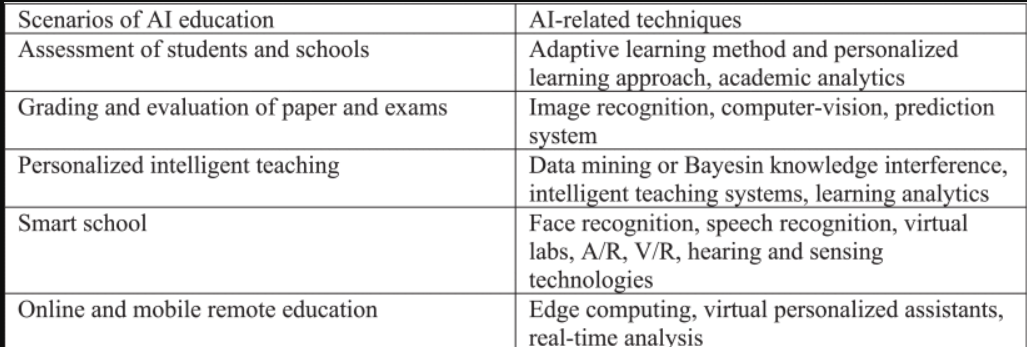
\includegraphics[scale=0.8]{figure1.png}
     \caption{Techniques for Scenarios of AI Education \cite{ArtificialInInEd}}
     \label{fig:enter-label}
 \end{figure}
\begin{comment}
    In questi ultimi anni innumerevoli sono state le sperimentazioni internazionali in cui l’Intelligenza Artificiale è stata utilizzata in campo educativo. Essa può essere utilizzata sia come argomento da studiare sia come stumento da usare.
    Noi ci concentremo sul secondo aspetto.

    Nella  figura Figure1 seguente potrai vedere i principali scenari dell'intelligenza artificiale nella vita degli studenti e le tecnologie a supporto di questi scenari.
    
\end{comment}

\newpage    %bibliografia

\bibliographystyle{plain}    %bibliografia
\bibliography{Bibliography.bib} %bibliografia



\end{document}  %Fine documento
